\documentclass[10pt,a4paper]{article}
\usepackage[utf8]{inputenc}
\usepackage[T1]{fontenc}
\usepackage{amsmath}
\usepackage{amssymb}
\usepackage{graphicx}
\usepackage{float}
\usepackage[english]{babel}
\title{Assignment \#7}
\author{Soulimane Mammar}
\begin{document}
	\maketitle
	
	\section*{Exercise 1}
	In this problem, you will model a circuit consisting of an arbitrary configuration of resistors. Provide a base class \verb|Circuit| with a member function \verb|get_resistance|. Provide a derived class \verb|Resistor| representing a single resistor. Provide derived classes \verb|Serial| and \verb|Parallel|, each of which contains a \verb|vector<Circuit*>|. A \verb|Serial| circuit models a series of circuits, each of which can be a single resistor or another circuit. Similarly, a \verb|Parallel| circuit models a set of circuits in parallel. For example, the following circuit is a \verb|Parallel| circuit containing a single resistor and one \verb|Serial| circuit.
	\begin{figure}[H]
		\centering
		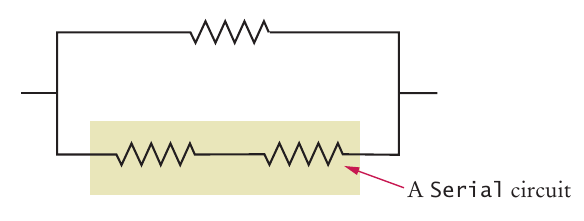
\includegraphics[width=0.7\linewidth]{circuit}
	\end{figure}
	
	\section*{Exercise 2}
	Part (a) of the figure below shows a symbolic representation of an electric circuit called an amplifier. The input to the amplifier is the voltage $ v_i $ and the output is the voltage $ v_o $. The output of an amplifier is proportional to the input. The constant of proportionality is called the “gain” of the amplifier. Parts (b), (c), and (d) show schematics of three specific types of amplifier: the \emph{inverting amplifier}, \emph{noninverting amplifier}, and \emph{voltage divider amplifier}. Each of these three amplifiers consists of two resistors and an op amp. The value of the gain of each amplifier depends on the values of its resistances. In particular, the gain, $ g $, of the inverting amplifier is given by $ g = -\dfrac{R_2}{R_1} $ . Similarly the gains of the noninverting  amplifier and voltage divider amplifier are given by $ g = 1 + \dfrac{R_2}{R_1}  $ and $g = \dfrac{R_2}{R_1+R_2}$, respectively.
	\begin{figure}[H]
		\centering
		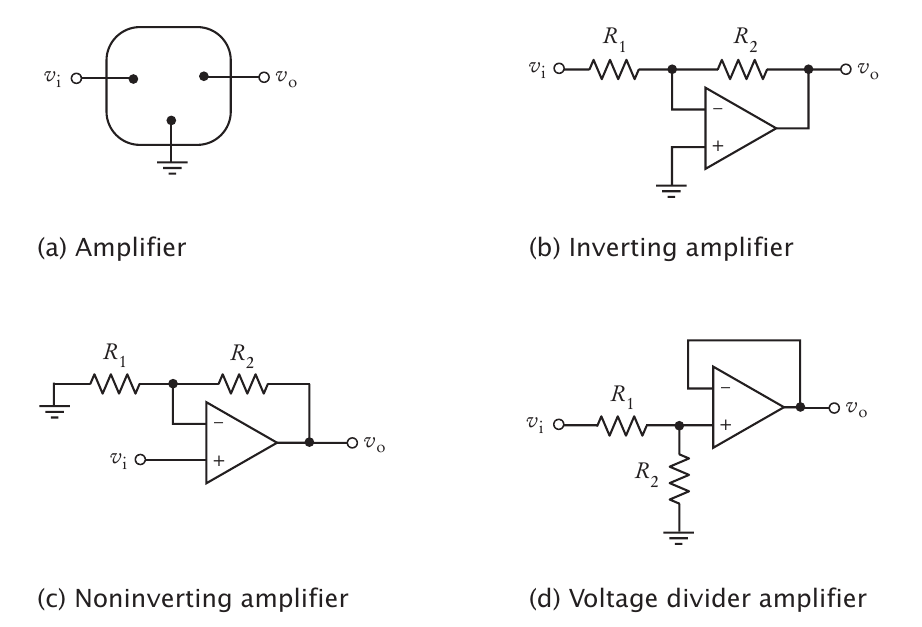
\includegraphics[width=0.7\linewidth]{amplifiers}
	\end{figure}
	
	Write a C++ program that represents the amplifier as a base class and represents the inverting, noninverting, and voltage divider amplifiers as derived classes. Give the base class two virtual functions, \verb|get_gain| and a \verb|get_description| function that returns a string identifying the amplifier. Each derived class should have a constructor with two arguments, the resistances of the amplifier. The derived classes need to override the \verb|get_gain| and \verb|get_description| functions of the base class. Write a main function for the C++ program that demonstrates that the derived classes all work properly for sample values of the resistances.
\end{document}